%% Material cut from gramsci_v2 (scope decision 2026-06-12):
%% the Quijote cosmology-response analysis, intended for a follow-up
%% paper. The measurements exist on disk:
%%   /home/csabiu/data/quijote/results/{Om,s8,h}_{m,p}_r*.{3pcf,4pcf}
%% (50 realisations per variation, fiducial x100 for errors), produced by
%% analysis/quijote/. Figures: quijote_{3pcf,4pcf}_responses.pdf.

\subsection{Response of the 3PCF and 4PCF to cosmological parameters}
\label{sec:responses}

Figures~\ref{fig:q3resp} and \ref{fig:q4resp} show the response of the
3PCF (equilateral and isoceles cuts) and 4PCF to each parameter pair,
$(\zeta_{+} - \zeta_{-})/\sigma_{\rm fid}$, expressed in units of the
single-realisation scatter so that the curves read directly as
per-configuration detectability for a $1\,(h^{-1}{\rm Gpc})^3$ volume.
(We normalise by the scatter rather than by $\zeta_{\rm fid}$ itself
because the fiducial 3PCF crosses zero, where fractional responses are
ill-defined.)

Two features stand out.  First, the responses of both statistics are
confined to quasi-linear scales: significant below
$r \approx 35\Mpch$ and consistent with zero above.  Second, the
parameter hierarchy is the same in both statistics:
$\Omega_{\rm m}$ produces the strongest response
(${\approx}1.5\,\sigma_{\rm fid}$ per configuration at
$r \approx 14\Mpch$ for the quoted step sizes), $h$ is comparable
(${\approx}1.1\,\sigma_{\rm fid}$), and $\sigma_8$ is markedly weaker
(${\approx}0.5\,\sigma_{\rm fid}$).  This ordering is the expected
consequence of the matched number density: a pure amplitude change
($\sigma_8$) is largely absorbed by the implied shift of the halo mass
threshold --- the familiar $\sigma_8$--bias degeneracy --- whereas
$\Omega_{\rm m}$ and $h$ alter the shape of the underlying power
spectrum (through $\Gamma \simeq \Omega_{\rm m} h$), which no threshold
adjustment can mimic.  The isoceles slice (bottom row of Figure~\ref{fig:q3resp}) shows the
same scale dependence and hierarchy at weaker per-configuration
amplitude, as expected for a cut whose sides sample lower-amplitude
separations.  The full measurements span all $1540$ (3PCF) and
$900$ (4PCF) configurations per realisation; the one-dimensional cuts
shown here are illustrative, and we emphasise that this is a qualitative
sensitivity demonstration rather than a Fisher forecast, which would
additionally require the full configuration covariance.

\begin{figure*}
\centering
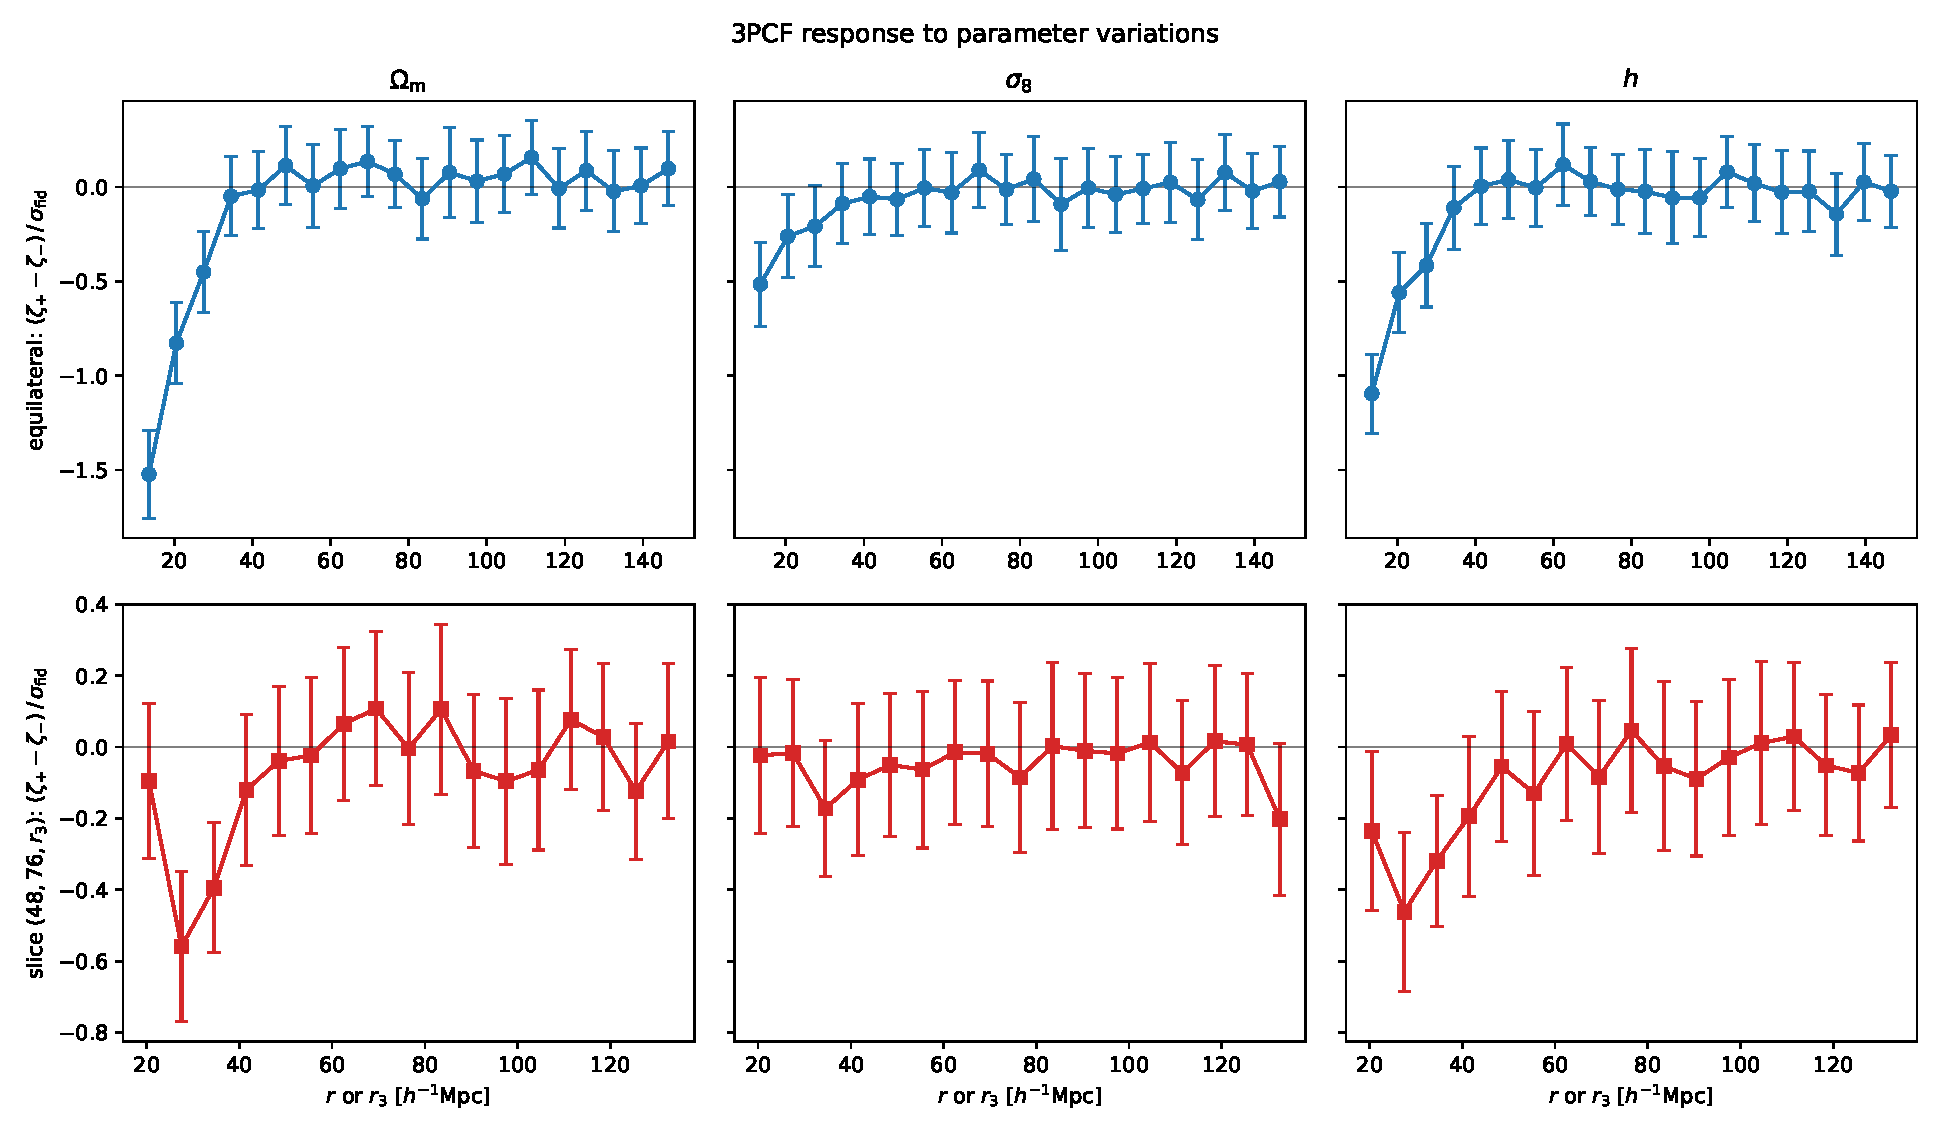
\includegraphics[width=0.92\textwidth]{figures/quijote_3pcf_responses.pdf}
\caption{Response of the 3PCF to the Quijote parameter variations, in
units of the single-realisation fiducial scatter, for the equilateral
cut (top row) and the isoceles slice $\zeta(48, 76, r_3)$ (bottom row).
Error bars propagate the ensemble errors of the variation means (50
realisations per side).  The responses are confined to quasi-linear
scales with the same parameter hierarchy in both cuts, and the matched
number density suppresses the $\sigma_8$ response relative to the shape
parameters $\Omega_{\rm m}$ and $h$ (see text).
\label{fig:q3resp}}
\end{figure*}

\begin{figure*}
\centering
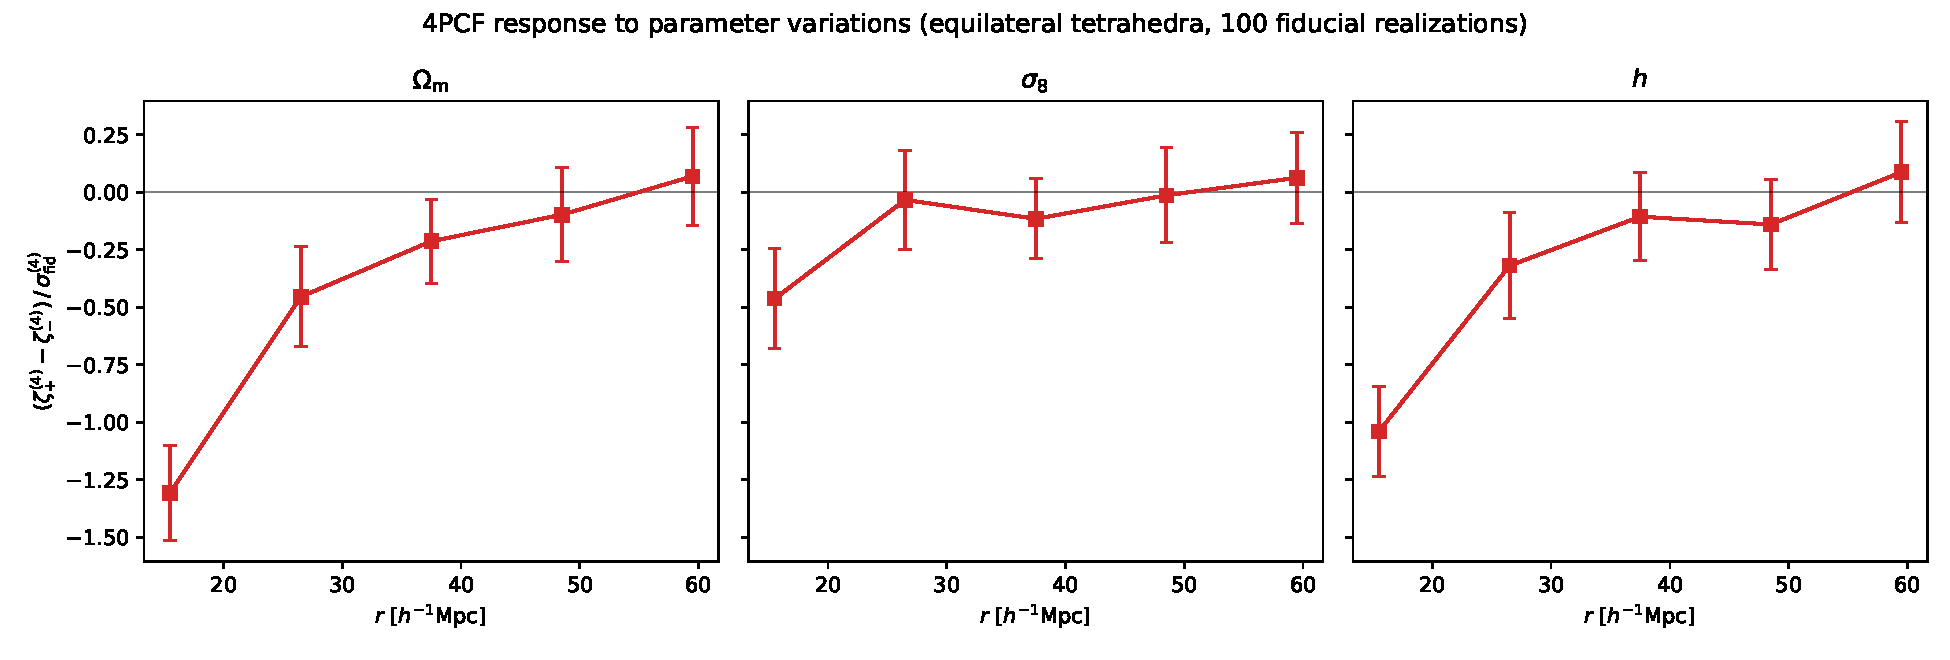
\includegraphics[width=0.92\textwidth]{figures/quijote_4pcf_responses.pdf}
\caption{As Figure~\ref{fig:q3resp}, for the connected 4PCF on
equilateral tetrahedra to $65\Mpch$.  The same scale dependence and
parameter hierarchy appear.
\label{fig:q4resp}}
\end{figure*}

